\chapter{Architecture} \label{architecture}

In this chapter we will present our suggested architecture for a hardware accelerated forward propagation of a Convolutional Neural Network used for recognizing handwritten digits. The architecuture will be presented in a top-down approach, starting with the topology and dataset of the network, followed by an overview of the software used, and finally, the hardware architecture of the accelerator. The source files for the VHDL and software code used in this project can for the time being be found at \cite{MyGithub}

\begin{figure}[h!]
  \centering
      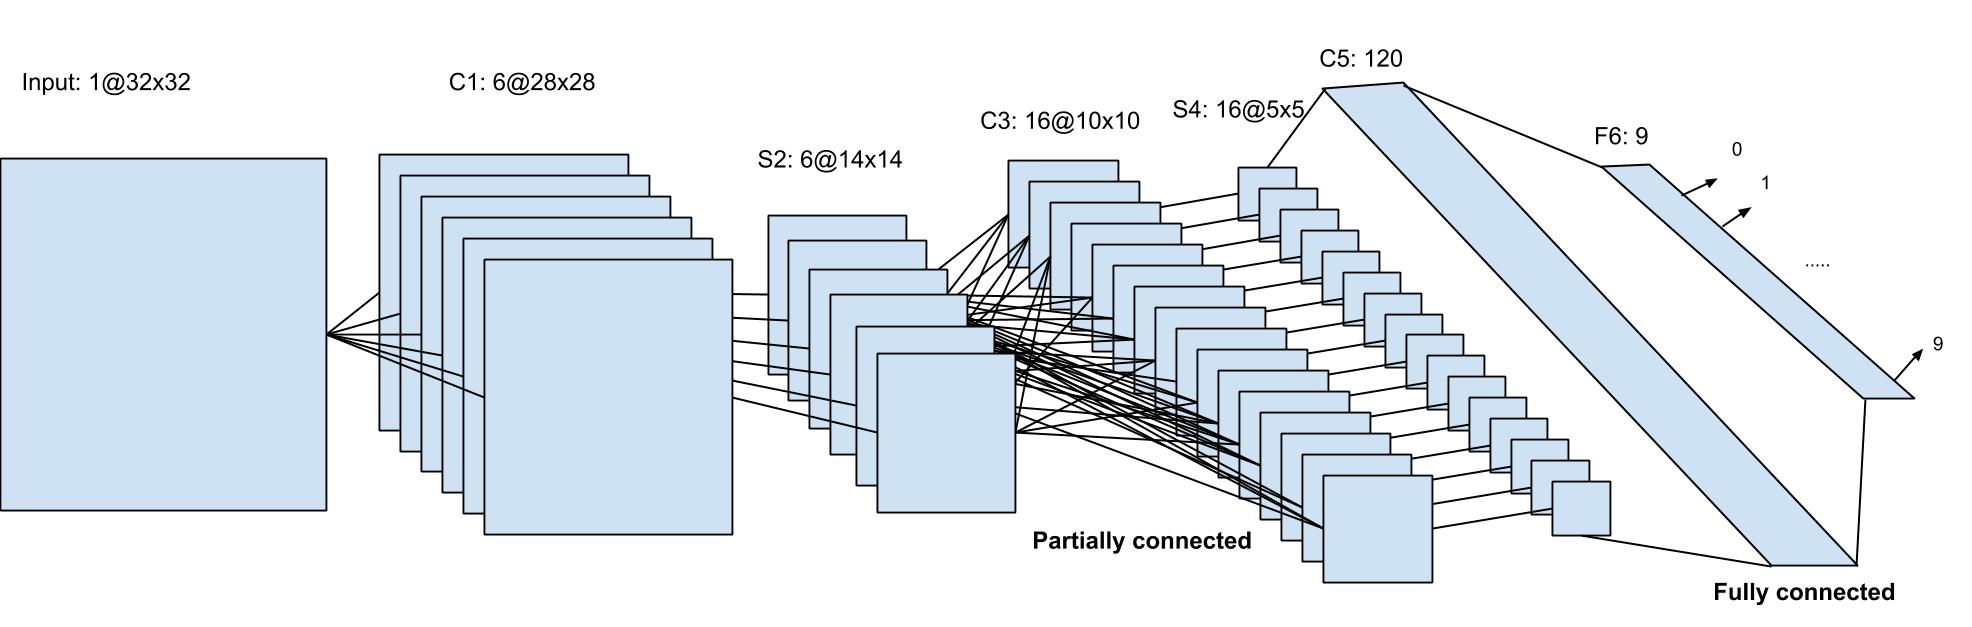
\includegraphics[width=1.2\textwidth, height=5cm]{Figures/Method/Network_topology}
    \caption{The topology of the implemented network.}
    \label{fig_network_topology}
\end{figure}

\section{Network Topology and Dataset}

We chose to implement a network with a smiliar topology as the LetNet-5 for digit recognition, as seen in Figure \ref{fig_network_topology}. It consist of six layers: 

\begin{itemize}
  \item \textbf{C1, convolution layer}. Takes in a single $ 32 \times 32 $ image of an digit. The image is convoluted using six different trained kernels, and outputs six respective $ 28 \times 28 $ feature maps. 
  \item \textbf{S2, subsampling/average-pooling layer.} Performs the subsample/average-pooling operation on each of the six $ 28 \times 28 $ feature maps from the previous layer, using a respective trained value for each map. The resulting output is six $ 14 \times 14 $ subsampled feature maps. 
  \item \textbf{C3, partially-connected convolution layer.} Takes in six $ 14 \times 14 $ feature maps which are partially connected to the sixteen $ 10 \times 10 $ output feature maps. These connections are shown in Table \ref{table_partial_connections}. The connections specifices which inputs are needed to compute a given output. E.g. in order to compute feature map 13, input 2, 4 and 5 are to be convoluted with the 13's kernel. The respective convoluted inputs are then combined into a single matrice, where a bias and activation function is applied to every element - which give the resulting output feature map. 
  \item \textbf{S4, subsampling/average-pooling layer.} Performs the subsample/average-pooling operation on each of the sixteen $ 10 \times 10 $ feature maps from the previous layer, using a respective trained value for each map. The resulting output is sixteen $ 5 \times 5 $ subsampled feature maps.
  \item \textbf{C5, fully connected convolution layer.} Takes in a sixteen $ 5 \times 5 $ feature maps which are fully connected to the 120 $ 1 \times 1 $ output feature maps. Since the size of the output feature maps are a single value, the feature maps are basically standard neurons. 
  \item \textbf{F6, output layer}. Takes in 120 neurons which are fully connected to the 10 output neurons. The output neuron with the highest value is the predicted value of the network. 
\end{itemize}


\begin{figure}[h!]
  \centering
      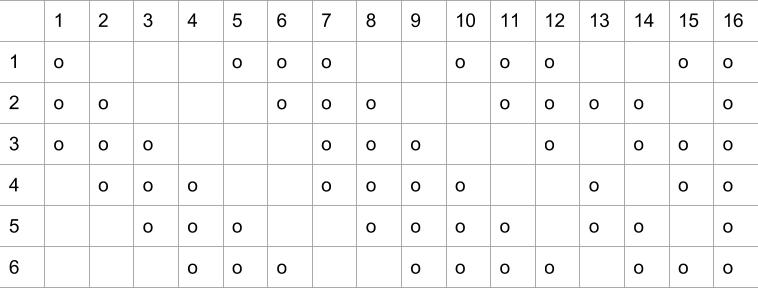
\includegraphics[width=1.0\textwidth]{Figures/Method/partial_connections}
    \caption{Table showing which of the six feature maps from S2 that are needed in order compute the feature maps of C3.}
    \label{table_partial_connections}
\end{figure}

There are three primary reasons for choosing this network. First, it is a relatively small network, which simplifies the implementation by reducing the chances of bugs and memory problems. Secondly, the kernel size of all the convolution layers are the same. This allowed for a less complex implementation, since we did not have to design our accelerator to support different kernel sizes, making it easier for the accelerator support all the convolution layers. Thirdly, this network have been shown to work very well with the MNIST dataset, i.e. our own experiments gave an accuracy of 99.1\%. Since the aim of this project is exploring hardware acceleration, we did not wish to spend time finding a working topology for a given dataset. Using a topology that has been shown to give high accuracy allowed us to focus more on acceleration rather than topology theory.   

 As mentioned, we used the \textit{the MNIST dataset}, available at \cite{MNIST}. It consists of 50 000 samples of handwritten digits ranging from 0-9, where 40 000 of the samples are used for
training and 10 000 samples are used to determine the accuracy of the network. 

\section{Write something about profiling and which parts I decided on accelerating}

Remember to quote newest LeChun article. 

\section{Software}

We have made extensive use of Taiga Nomi's C++ framework for neural networks, available at \cite{SoftwareGithub}, in our project. The framework was used in order to train the parameters of our network, for measuring the efficency of a pure software implementation, and as a basis for the implementation that uses the hardware accelerator. The framework treats each layer in the network as a seperate software module, which makes it easy to swap diffrent implementations of a layer. This simplified the process of integrating the hardware accelerator into the network, since we could simply exchange the original modules with our own.

Figure \ref{fig_software_architecture} A shows a simplified version of the architecture of the pure software implementation of our network. Each layer contains a set of pretrained weights which are loaded before the network starts processing the images. When an image is inputted to the first layer, it performs the calculations described in Chapter \ref{chap_background} in software, and propegates the result to the next layer. 

Figure \ref{fig_software_architecture} B shows how the original software was changed in order to make use of the accelerator. As mentioned, we decided to accelerate the convolutional layer and the subsample/average-pooling layer, thus we wrote a new software module that would handle both operations. But instead of computing the operations in software, the new module transfer the input data and the weight to the hardware accelerator and extracts the result from the computations. 

We decided against accelerating layer C5. The main reason being that in its current form, the accelerator is only able to compute one feature map at a time. Each computation comes with a certain amount of overhead, i.e. transfering data to/from the accelerator and configuring it. Thus for C5, which takes in 120 $ 5 \times 5 $ matices, we figured that input was so numerous and so small that it would cause too much overhead in order to be efficient. Though this is mostly guesswork, and should be tested before any absolute conclusion is reached. But due to lack of time, this was saved for future work. 


\begin{figure}[h!]
  \centering
      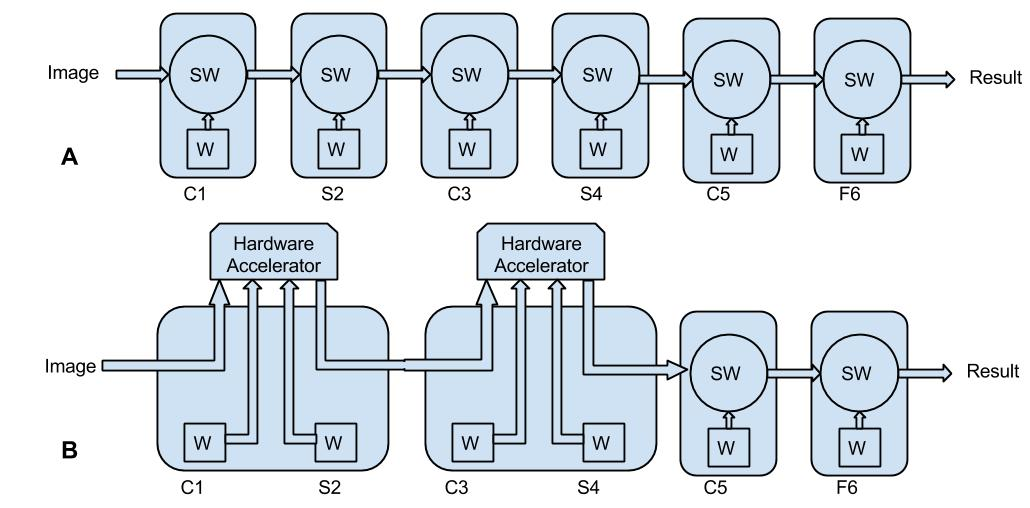
\includegraphics[width=1.0\textwidth]{Figures/Method/SoftwareArchitecture}
    \caption{A simplified overview of the software architecture with and without hardware acceleration.}
    \label{fig_software_architecture}
\end{figure}

\subsection{Hardware driver}

A driver for the accelerator was written in order to create a simple and easy to use interface to the hardware. As mentioned, the accelerator can only compute on feature map at a time, thus the input to the driver is all the data required to compute said feature map. That is, a set of images, their respective kernels and bias, the average pooling constant and its respective bias. The driver then feeds this data to the accelerator, and returns the computed feature map. 

In order to control the accelerator, the driver accesses two memory-mapped control registers. The first registers is used to set which layer is currently going to be processsed, i.e. C1/S2 or C3/S4, and the second one is used to start the accelerator when the input data is ready. 

For data transfer the driver uses a \textit{direct memory access controller} (DMA) IP from Xilinx. This is where most of work on the driver had to be done, since the DMA interface is much more complex compared to the accelerator interface. The DMA is configured to transfer the weights and image(s) to the accelerator's input buffer, and extract the data from the output buffer. Since the output buffer is a FIFO, the DMA is able to extract each output value as they are produced, instead of waiting for the accelerator to finish and then transfer all the output data. 


\begin{figure}[h!]
  \centering
      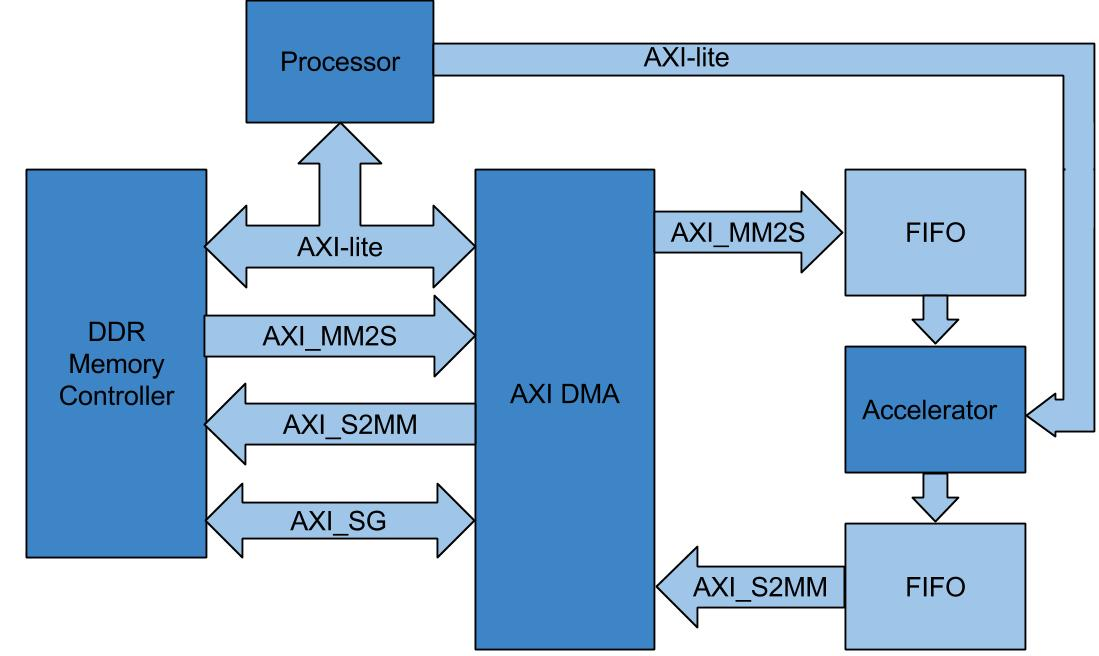
\includegraphics[width=0.5\textwidth]{Figures/Method/DriverAcceleratorInteraction}
    \caption{The interaction between the driver, DMA and accelerator.}
    \label{fig_driver_acc_interact}
\end{figure}
 

\section{Hardware}

In this section we will describe the hardware architecture of the system as a whole, and more specifically, our accelerator. Do note that the descriptions and the figures are simplified to some extent. This simplication is done with the intent of not making the description and explainations too complex. We rather focus on conveying the important ideas of the design, instead of describing the implementation to the last detail. 

\subsection{Overview of hardware achitecture}


\subsection{Accelerator Interface}

The accelerator has three bus interfaces that are used to control it. The first is a slave \textit{Advanced eXtensible Interface} (AXI) interface which is used to write the two control registers, and reading a set of status registers of the accelerator. The status registers are mostly used for debugging, i.e. reading various crucial values inside the accelerator, but also to determine whether the accelerator is currently processing. The bus is connected to the ARM processor, to allow direct communication between software and hardware.

The second bus interface is a slave \textit{AXI-Streaming} (AXIS) interface, which is used to stream the data input into the accelerator. The interface is connected to a \textit{first-in-first-out} (FIFO) buffer, where all the data required by the accelerator is stored until the accelerator is ready to consume them. 

The third bus interface is a master AXIS interface, which is connected to another FIFO buffer. The computed feature map is streamed out of the accelerator into the buffer, and stored there until the DMA is able to move the data back to software control.

 



\subsection{Accelerator Internal}

As previously stated, the accelerator takes \textit{n} images as input, $ I_1, I_2, \dots, I_n $, n respective kernels $ K_1, K_2, \dots, K_n $, two biases, and outputs a single processed image $ O $. Using the input images, the kernel and the bias, it performs the operations of the convolution and subsampling/pooling layer for a single feature map. Thus the output $ O $ is a subsampled/pooled feature map that has been produced by convoluting the images $ I_1, I_2, \dots, I_n $ with the kernels $ K_1, \dots, K_n $. 

The accelerator can thus compute the whole convolution and subsample/pooling layer by doing the above computations for all the output feature maps in the layer. One can exploit inter-parallelism by making several instances of the accelerator run in parallel. One can also exploit intra-parallelism, but then one need to connect the different accelerator instances so they can add up the results from the convolutions without using the intermediate convolution buffer, as described in \cite{Chakradhar2010}. Unfortunately, within the given timeframe we were unable to get a system working that exploited inter- and intra parallelism. But the architecture is designed to be easily extendable to support this, given more development time. 


The accelerators consists of five major components (Figure \ref{fig_imagezor_architecture}):

\begin{itemize}
	\item \textbf{The convoluter}. Performs the convolution operation on the input.
	\item \textbf{The intermediate convolution buffer}. Since the resulting feature map is the sum of the convolutions of all the input images (with the exception of the first layer), this buffer is needed to store the results from the previous convolution, so that it can be accumulated with the current convolution. In the first layer of the network there is only one input image (i.e. $ n = 1 $), thus no summation is needed.
	\item \textbf{Tanh}. Performs the non-linear hyperbloc tangent function  on the feature maps.
	\item \textbf{Subsample/average-pooler}. Performs the subsample/average-pool operation on the feature maps. 
\end{itemize}

\begin{figure}[h!]
	\centering
    	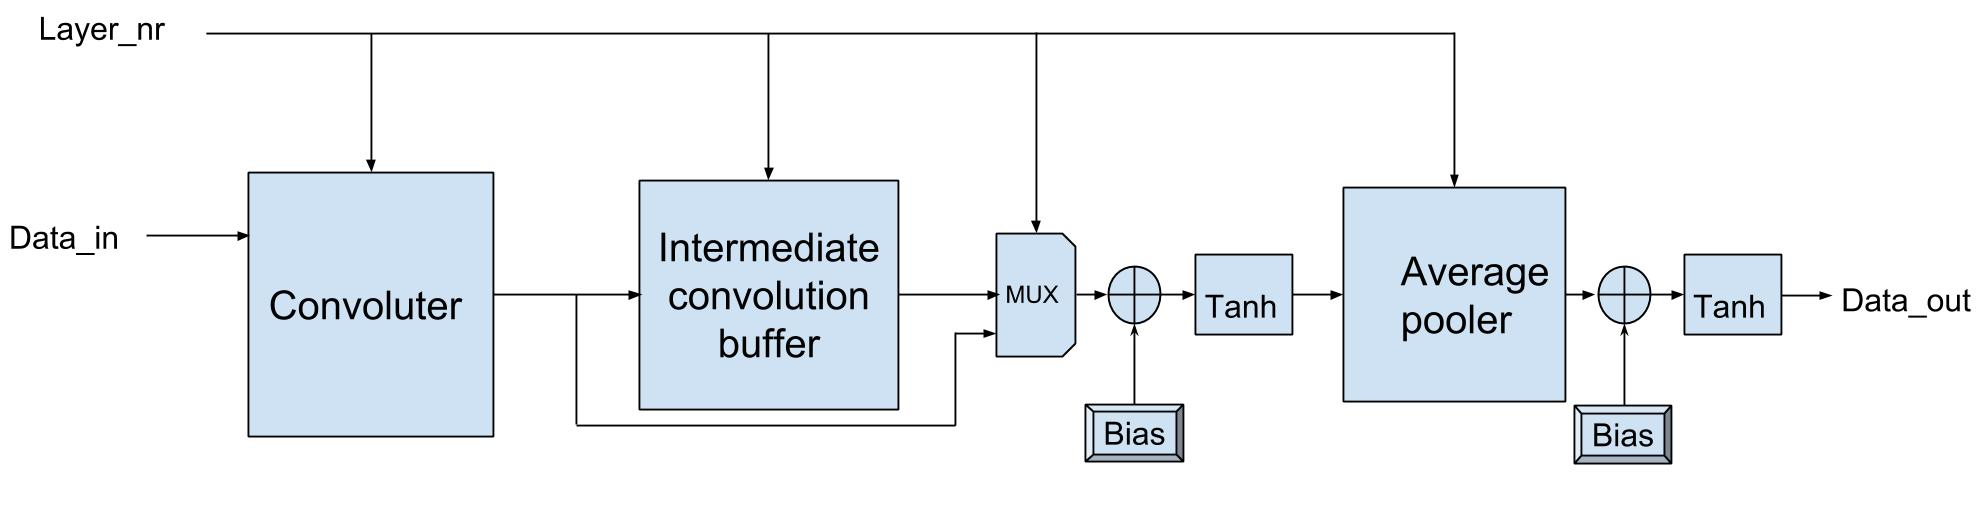
\includegraphics[width=1.0\textwidth]{Figures/Method/conv_layer_arch}
  	\caption{The architecture of Imagezor.}
  	\label{fig_imagezor_architecture}
\end{figure}

The \textit{layer\_nr} signal is used to define if it is C1/S2 or C3/S4 that is being computed. The input image(s) in the first layer is bigger than in the second ($ 32 \times 32 $ vs $ 14 \times 14 $), which the convoluter and the average pooler need to compensate for (see Section \ref{sec_convoluter} and \ref{sec_average_pooler}). In addition in the second layer the intermediate convolution buffer needs to be activated so it accumulate and store all the convolutions needed to compute a single feature map. Thus the mux is needed to propagate the data directly from the convoluter for C1/S2, and from the buffer for C3/S4. 


In order to reduce resources spent and execution time, the accelerator uses Q16.16 fixed-point arithmetic, which is shown to give virtually the same network accuracy as floating-point arithmetic\cite{Napocensis2009} \cite{Holt1993} \cite{Chen2014}. Something that our own experiments also shows.  

In the sections below we will provide a more detailed description of the convoluter, the hyperbolic tangent unit and the average pooler. 


\subsection{The Convoluter} \label{sec_convoluter}

This module is inspired by \cite{Farabet2009}. The input is a $ n \times n $ image, and the output is a $ (n-k+1) \times (n-k+1) $ feature map, using a $ k \times k $ kernel. The kernel is stored in internal registers that must be rewritten for each different feature map that is to be computed. Every clock cycle the module takes in a pixel as input, and after a certain delay it will output a processed pixel almost every cycle. Each pixel is inputted once, left to right, one row at a time. 

It consists of 2D grid of multiply and accumulate (MAC) units which represents the convolution kernel. Thus the grid dimension is equal to the kernel dimension. In every MAC unit there is a register that contains the respective kernel weight. In every clock cycle the MAC units multiply the input pixel with its weight, and then accumulates the result from the previous cycle of the MAC unit to the left. 

At the end of each row of MACs there is $ n - k $ shift registers. The result of the last MAC in each row is stored in the first shift register, and the first MAC in each row takes the value of the last shift register of the previous row as accumulation input. The exception being the absolute first and last MAC unit. Every clock cycle the values in the shift registers are shifted to the right. 

\begin{figure}[h!]
  \centering
      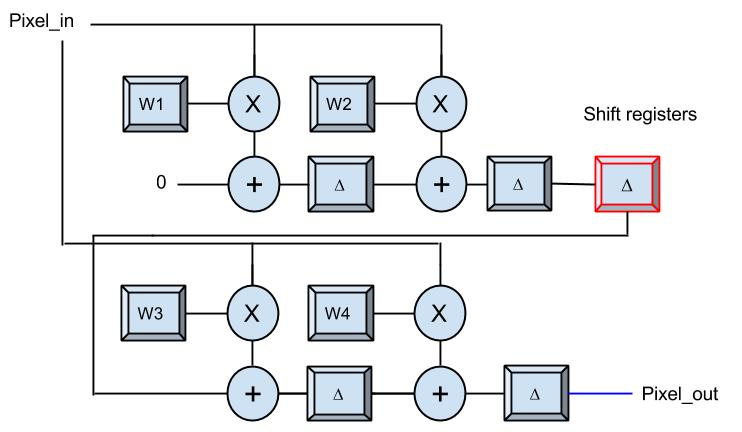
\includegraphics[width=0.7\textwidth]{Figures/Method/Convolver}
  \caption[The convoluter ]{The convoluter, when $ n = 3 $ and $ k = 2 $.}
\end{figure}
	
By providing this delay you only have to input each pixel once during the convolution. Generally every pixel is needed for $ k \times k $ convolution operations (the exception being the pixels close to the boarders of the image). Thus the shift registers are used to store the intermediate values of the convolutions until a pixel that is needed for the respective convolution operation is inputted. 

The delay these shift registers cause are the reason for the delay before valid output pixels are produced. Thus from when the convolution starts, the output will not be valid before $ k-1 $ rows of the image have been processed. And for every new image row, there will be a $ k-1 $ cycle delay before the output is valid. This is demonstrated by the fact that the input image is a $ n \times n $ matrix, while the output matrix is a $ (n-k+1) \times (n-k+1) $ matrix. 

Since the two layers in the network have different image sizes, but uses the same kernel size, we can reuse the module for both of them. This is done by having the control signal \textit{layer\_nr} decide how many of the shift registers that are to be used during convolution. In the first layer all of the shift registers are used, but in the second only a subset is used. I.e. $ n-k+1 $ of shift registers are used in each row, where $ n $ is either 32 or 14. 

The loading of the weights takes $ k \times k $ clock cycles, and the processing of the image takes $ n \times n $ clock cycles. Thus the total number of cycles it takes to perform a full convolution of an image is $ n \times n + k \times k $. But based upon the papers refered to in Section \ref{chap_related_work} it seems that \textit{n} tends to be larger than \textit{k}. E.g. for the first layer in the LeNet-5 \cite{LeCun1998}, $ n = 32 $ and $ k = 5 $, the loading  of the weights take 25 clock cycles and the image processing 1024 cycles. This means that the execution time of the convoluter is primairly bounded by the size of the image. But the size of the kernel decides the hardware resource cost of the module, since it requires $ k \times k $ DSP slices on the FPGA.

\begin{figure}[h!]
  \centering
      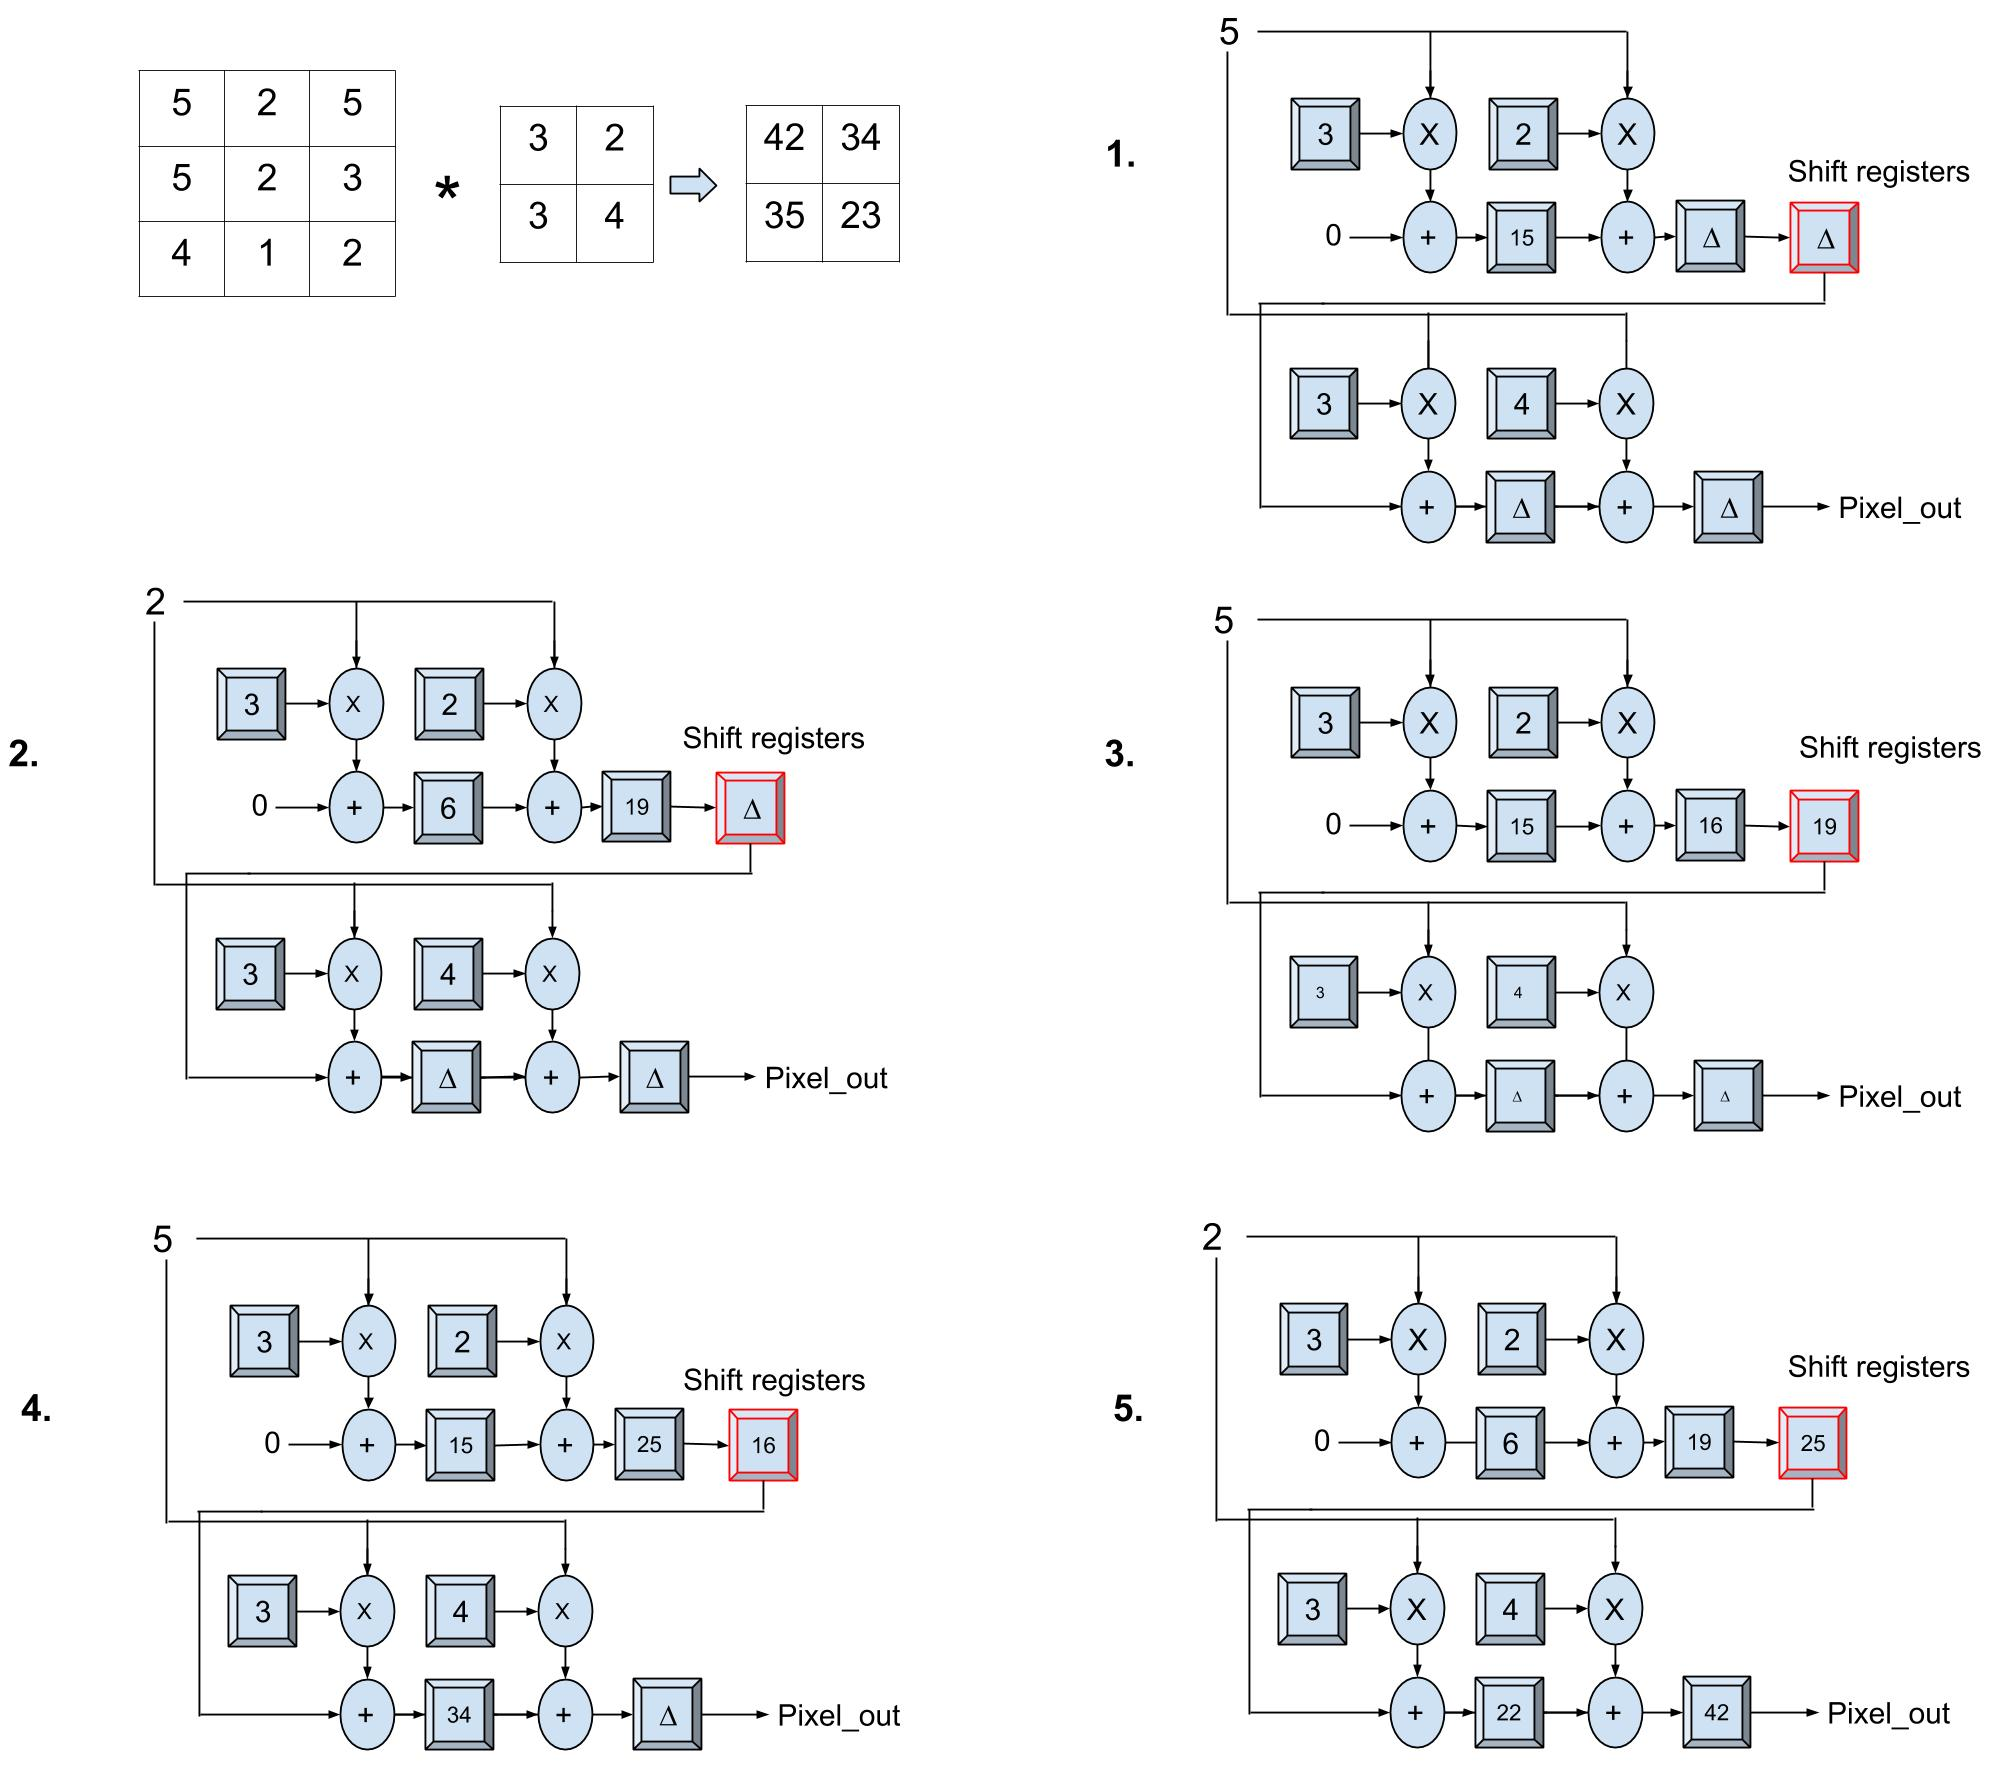
\includegraphics[width=1.1\textwidth]{Figures/Method/Conv_example}
  \caption[Convolution example]{Example showing the five first clock cycle of an convolution. The weights of the kernel is already loaded into the MAC units, and every cycle a new pixel from the image in inputted. In the last example you can see that 42 is provided as the first output.}
\end{figure}

\subsection{The Hyperbolic Tangent} 

This module is based upon \cite{XXXXXXXXXX} using \textit{piecewise linear approximation}. It takes input a single value \textit{x} and outfputs a linear approximation of the hyperbolic function. Using a lookup table (Table \ref{tab_tanh}) and the constants from Table \ref{tab_tanh_constants} the module decides which linear approximation to use. 
In order to meet the timing constraints on the FPGA the module has a pipeline length of three. 

\begin{table}
	\centering
    \begin{tabular}{| >{\centering\arraybackslash}m{1.2in} |} 
    \hline
    Constants \\ \hline
    $ m_1 = -0.54324 $ \\ \hline
    $ m_2 = -0.16957 $ \\ \hline
    $ c_1 = 1 $ \\ \hline
    $ c_2 = 0.42654 $ \\ \hline
    $ d_1 = 0.016 $ \\ \hline
    $ d_2 = 0.4519 $ \\ \hline
    $ a = 1.52 $ \\ \hline
    $ b = 2.57 $ \\ \hline
        \end{tabular}
    \caption{The constant used for the hyperbolic tangent approximation.}
   	\label{tab_tanh_constants}
    
	\centering
    \begin{tabular}{| >{\centering\arraybackslash}m{1.2in} | >{\centering\arraybackslash}m{2.5in} |} 
    \hline
    Conditions & Output \\ \hline
    $ 0 \le |x| \le a $ & $ sign(x) \times [0.5 \times m_1 \times |x|^2 + c_1 \ times |x| + d_1] $\\ \hline
    $ a \le |x| \le b $ & $ sign(x) \times [0.5 \times m_2 \times |x|^2 + c_2 \ times |x| + d_2] $\\ \hline
   	$ otherswise $ & $ signed(x) $\\ \hline
        \end{tabular}
    \caption{The piecewise linear approximation of the hyperbolic tangent.}
   	\label{tab_tanh}
    
\end{table}

\vspace*{1\baselineskip}
\subsection{The Average Pooler} \label{sec_average_pooler}

The max pooler performs the subsample/max-pooling operation described in Section \ref{sec_cnn_def}. The input is a $ (n-k+1) \times (n-k+1) $ feature map, and the output is a $ (n-k+1)/p \times (n-k+1)/p $ subsampled/max-pooled feature map, where \textit{p} is the dimension of subsample neighborhood. As with the convoluter, one pixel is streamed in every cycle, and streamed out whenever a valid pixel is ready. Designed this way the max pooler can process in parallel with the convoluter, by directly streaming the output of the convoluter into the max pooler module. In other words, the operations of convolution layer and subsampling/pooling layer is pipelined.

\begin{figure}[h!]
  \centering
      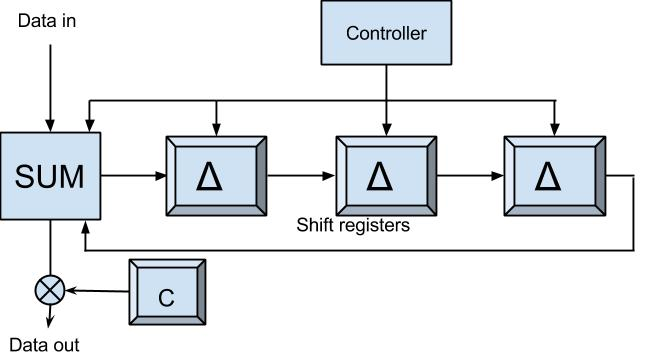
\includegraphics[width=0.5\textwidth]{Figures/Method/submax}
  \caption{The average pooler.}
\end{figure}

The module compares the input with the current max value, and updates the max value accordingly. It contains a set of \textit{(n-k+1)/p} shift registers. Since the image is divided into $ p \times p $ non-overlapping neighborhoods, the module needs to store the current maximum value of previous neighborhood when a pixel from a new neighborhood is inputted. To do this the module contains two counters, \textit{row\_num} and \textit{column\_num}. When a new pixel is inputted the \textit{column\_num} counter is incremented, and when a new row is encountered the \textit{row\_num} counter is incremented. Every time $ column\_num~mod~p = 0 $ the shift registers are shifted one to the right, and every time $ column\_num~mod~p = 0 $ and $ row\_num~mod~p = 0 $ a valid output is produced. 



The execution speed of the max pooler module is bounded by the size of the feature map, $ (n-k+1) \times (n-k+1) $ clock cycles, finishing one cycle after the last pixel has been inputted. 
Thus by streaming the output of the convoluter to the max pooler, both will finish only a few cycles apart, effectively running both jobs in parallel. The resource usage of the module is bounded by the size of the subsampling dimension, since it requires a number of shift registers equal to the size of the dimension. But essentially its resource usage is quite low.  
